\chapter{Практическое задание}

\section{Некоторые флаги системного вызова open()}
\begin{itemize}
	\item O\_CREAT -- создание обычного файла, если его нет.
	\item O\_EXCL -- при использовании с O\_CREAT open() выдаст ошибку.
	\item O\_APPEND -- открытие файла в режиме добавления в конец. При это файловый указатель будет смещен на конец при каждой операции записи.
	\item O\_LARGEFILE -- позволяет открывать файлы, размер которых не может быть представлен off\_t.
	\item O\_PATH -- получение файлового дескриптора, который может быть использован в двух случаях: указать местоположение в файловой системе или выполнить операции на уровне файлового дескриптора (close(), fchdir(), fstat() и т.д)
	\item O\_SYNC -- операции по записи в файл будут завершены в соответствие с требованиями синхронизированного ввода-вывода.
	\item O\_TMPFILE -- создание безымянного временного обычного файла.
	\item O\_TRUNC -- содержимое файла будет очищено, при этом сам файл не удаляется (если он существует и есть права на запись).
\end{itemize}

\section{Алгоритм выполнения системного вызова open()}
Ниже на рисунке \ref{image:open} представлена схема алгоритма системного вызова open() на верхнем уровне. Различные функции, вызываемые внутри него представлены на рисунках \ref{image:build_open_flags}, \ref{image:get_name_flags}, \ref{image:alloc_fd}, \ref{image:do_filp_open_1}, \ref{image:do_filp_open_2}, \ref{image:do_open_1}, \ref{image:do_open_2}, \ref{image:do_last_lookups}.
\newpage
\begin{figure}[H]
	\captionsetup{justification=centering}
	\centering{
		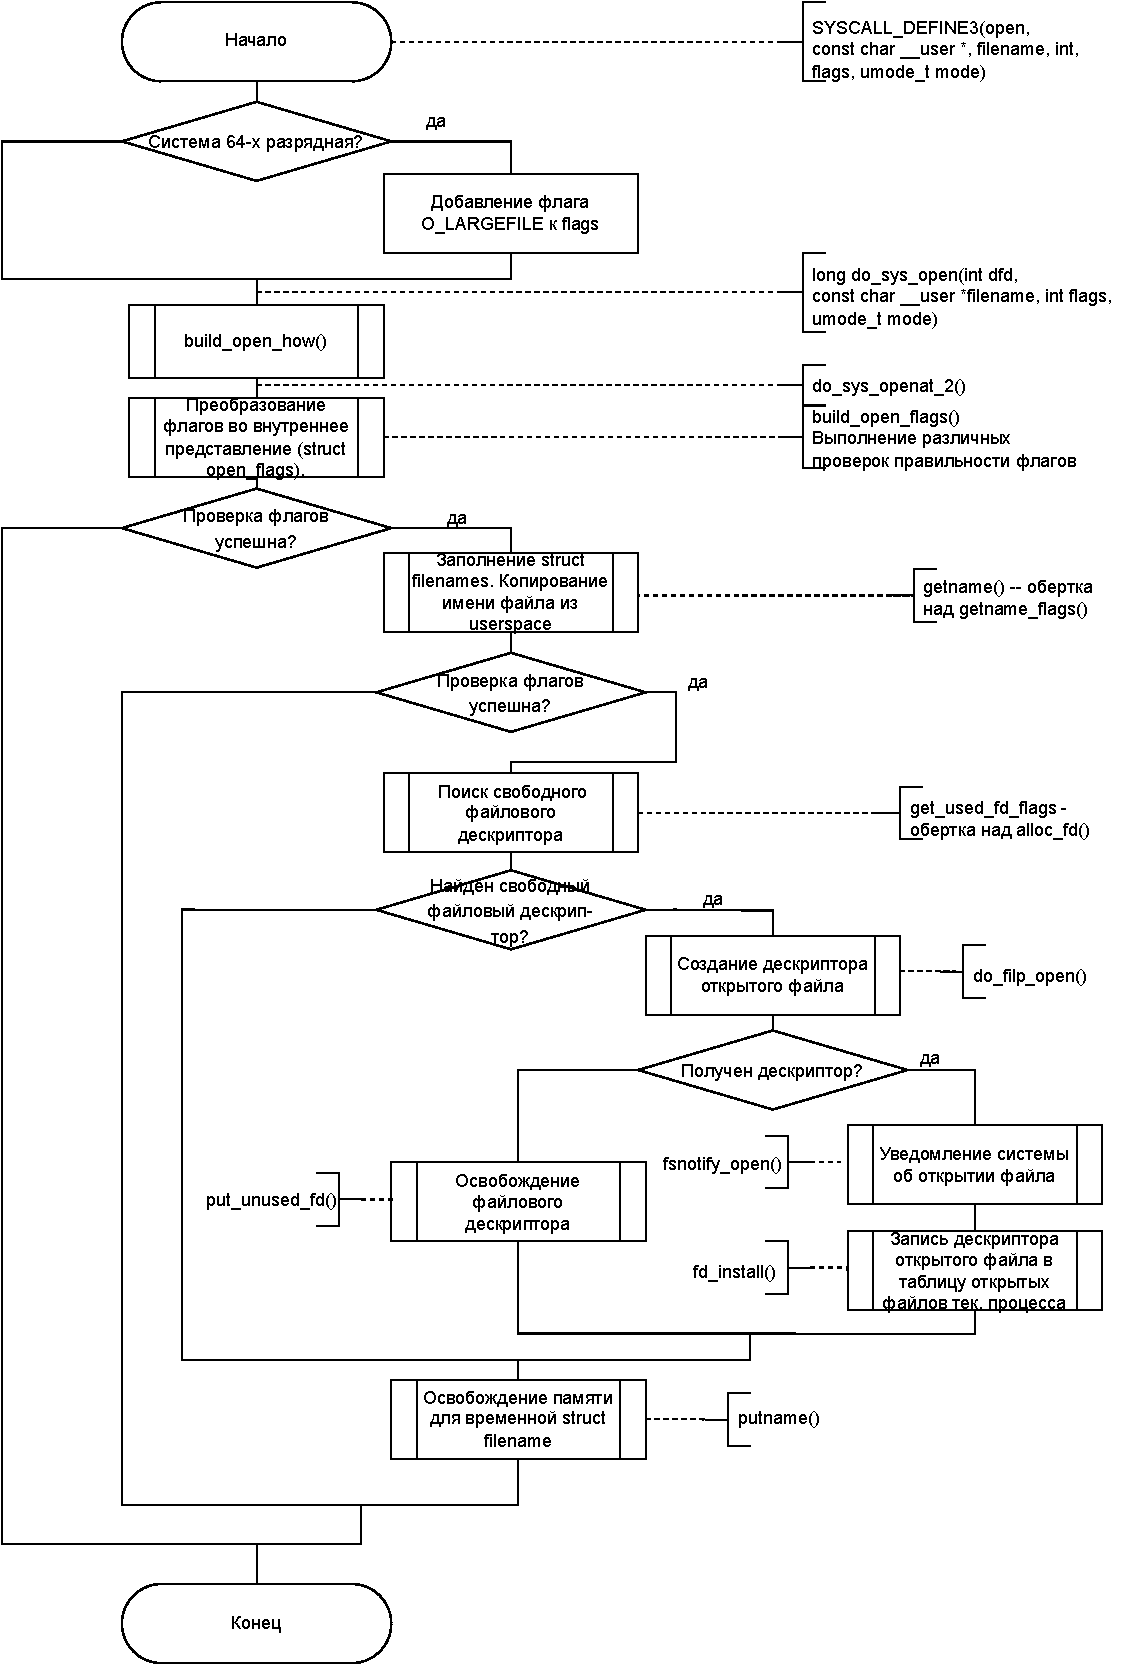
\includegraphics[scale=0.9]{images/open.pdf}
		\caption{Схема алгоритма системного вызов open()}
		\label{image:open}
	}
\end{figure}

\begin{figure}[H]
	\captionsetup{justification=centering}
	\centering{
		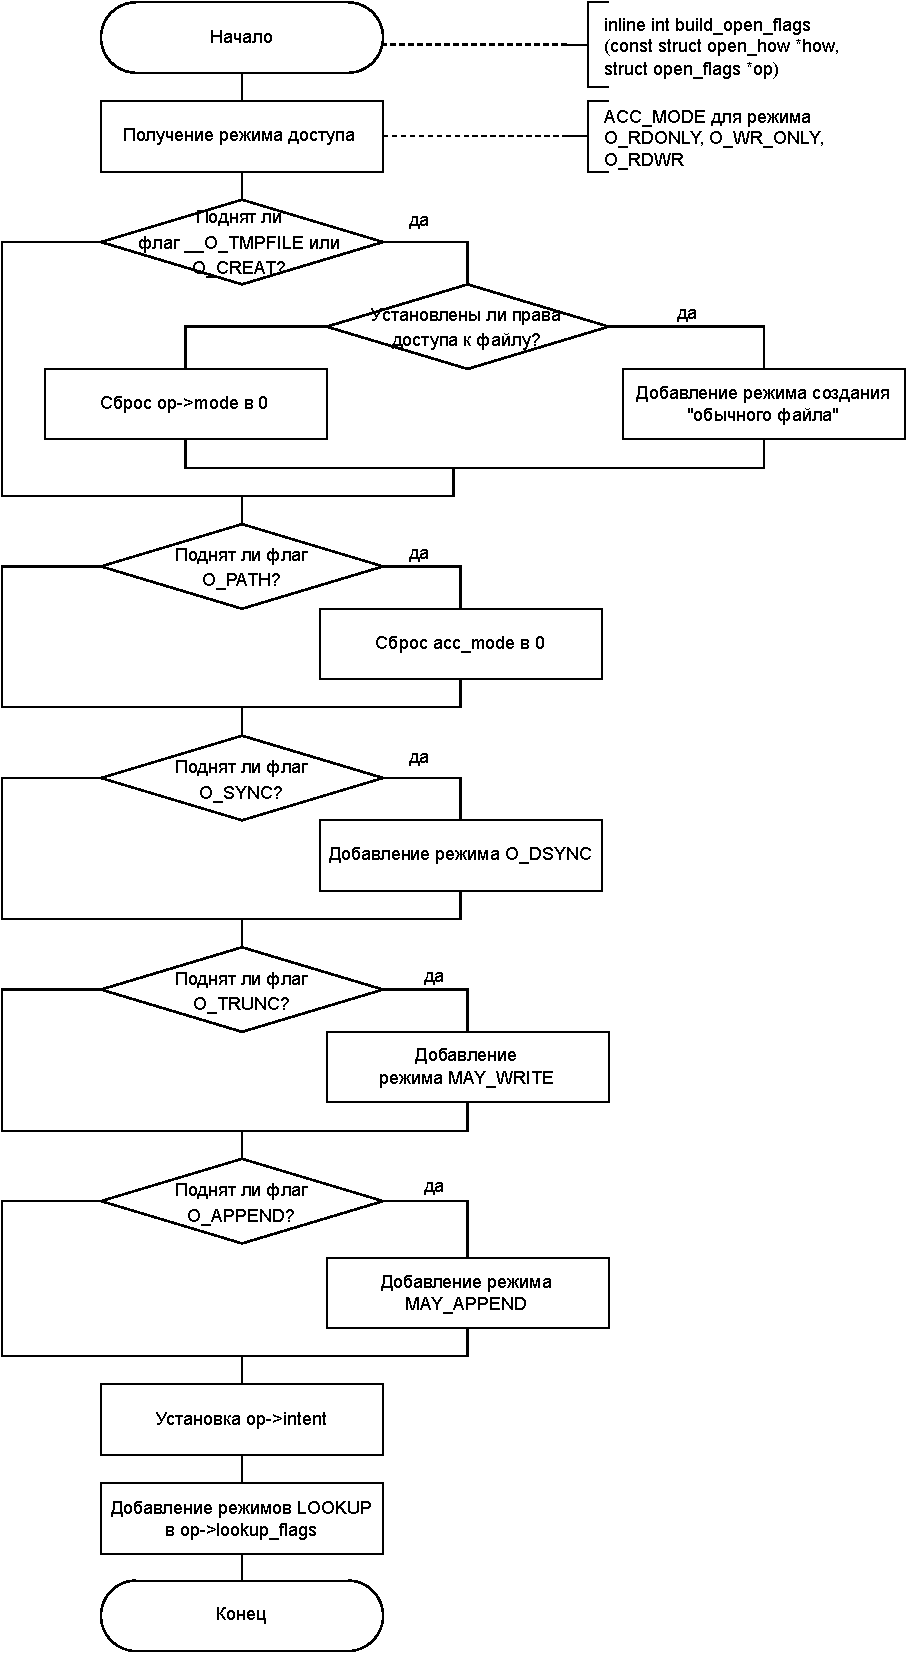
\includegraphics[scale=0.9]{images/build_open_flags.pdf}
		\caption{Схема алгоритма функции build\_open\_flags()}
		\label{image:build_open_flags}
	}
\end{figure}

\begin{figure}[H]
	\captionsetup{justification=centering}
	\centering{
		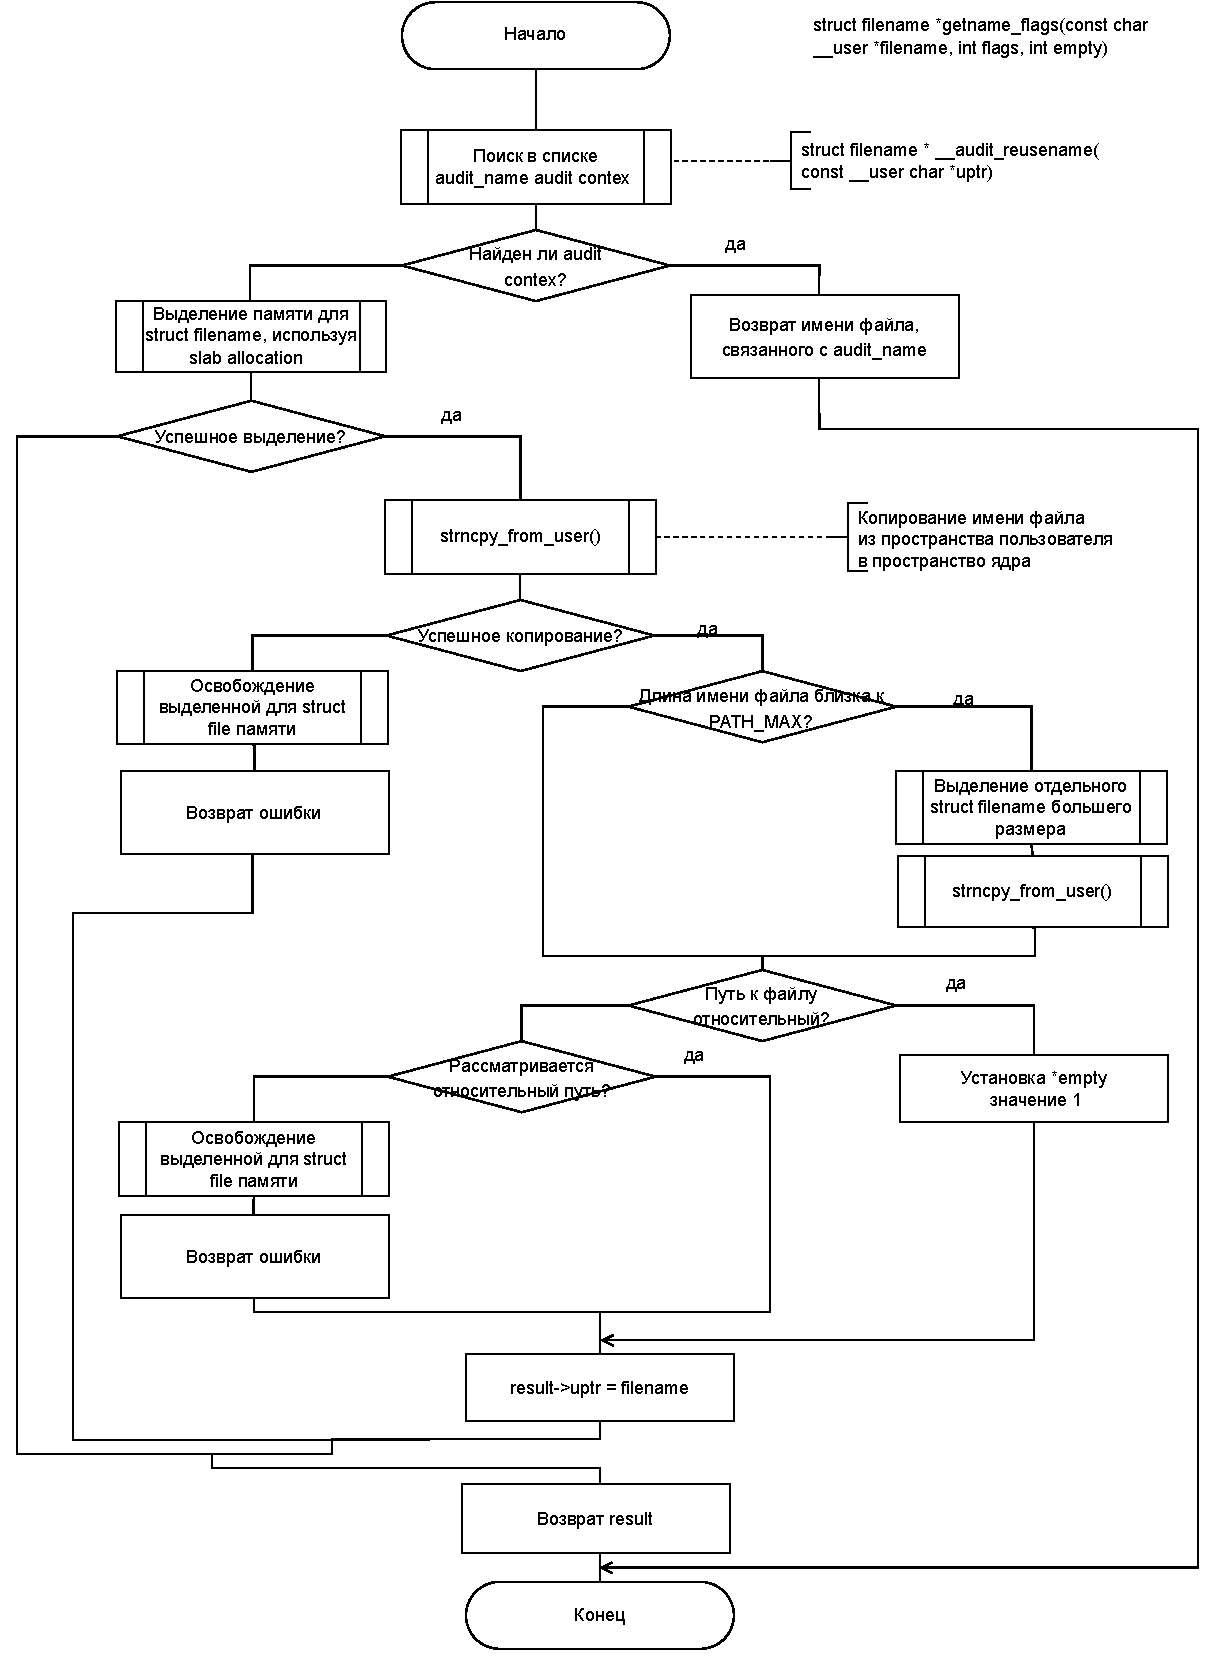
\includegraphics[scale=0.85]{images/getname_flags.pdf}
		\caption{Схема алгоритма функции getname\_flags()}
		\label{image:get_name_flags}
	}
\end{figure}

\begin{figure}[H]
	\captionsetup{justification=centering}
	\centering{
		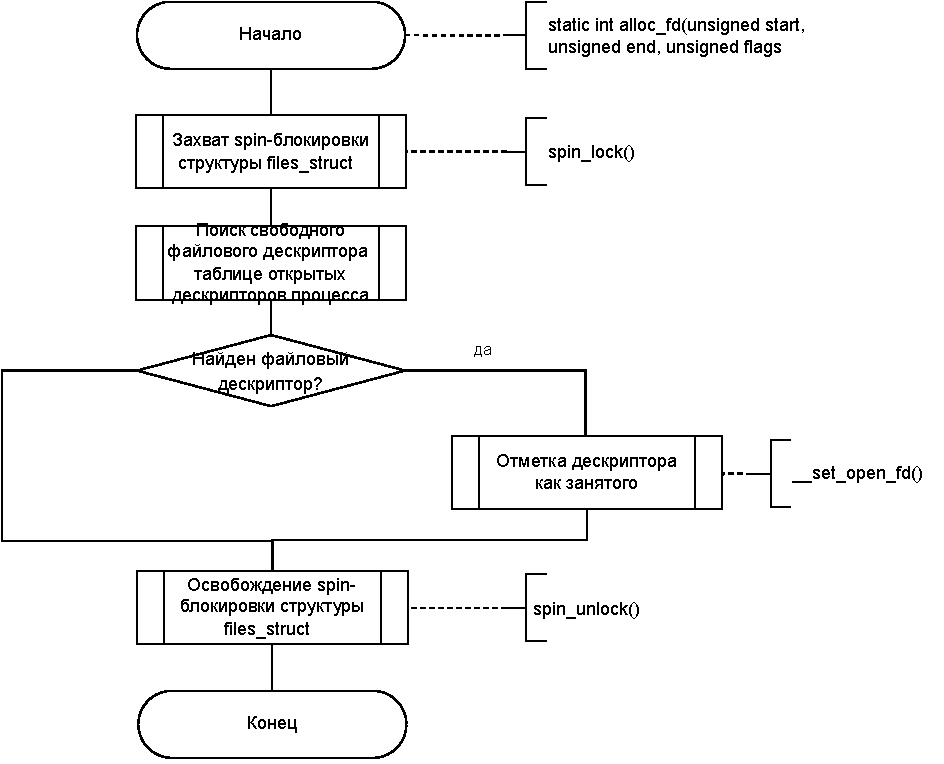
\includegraphics[scale=0.9]{images/alloc_fd.pdf}
		\caption{Схема алгоритма функции alloc\_fd()}
		\label{image:alloc_fd}
	}
\end{figure}

\begin{figure}[H]
	\captionsetup{justification=centering}
	\centering{
		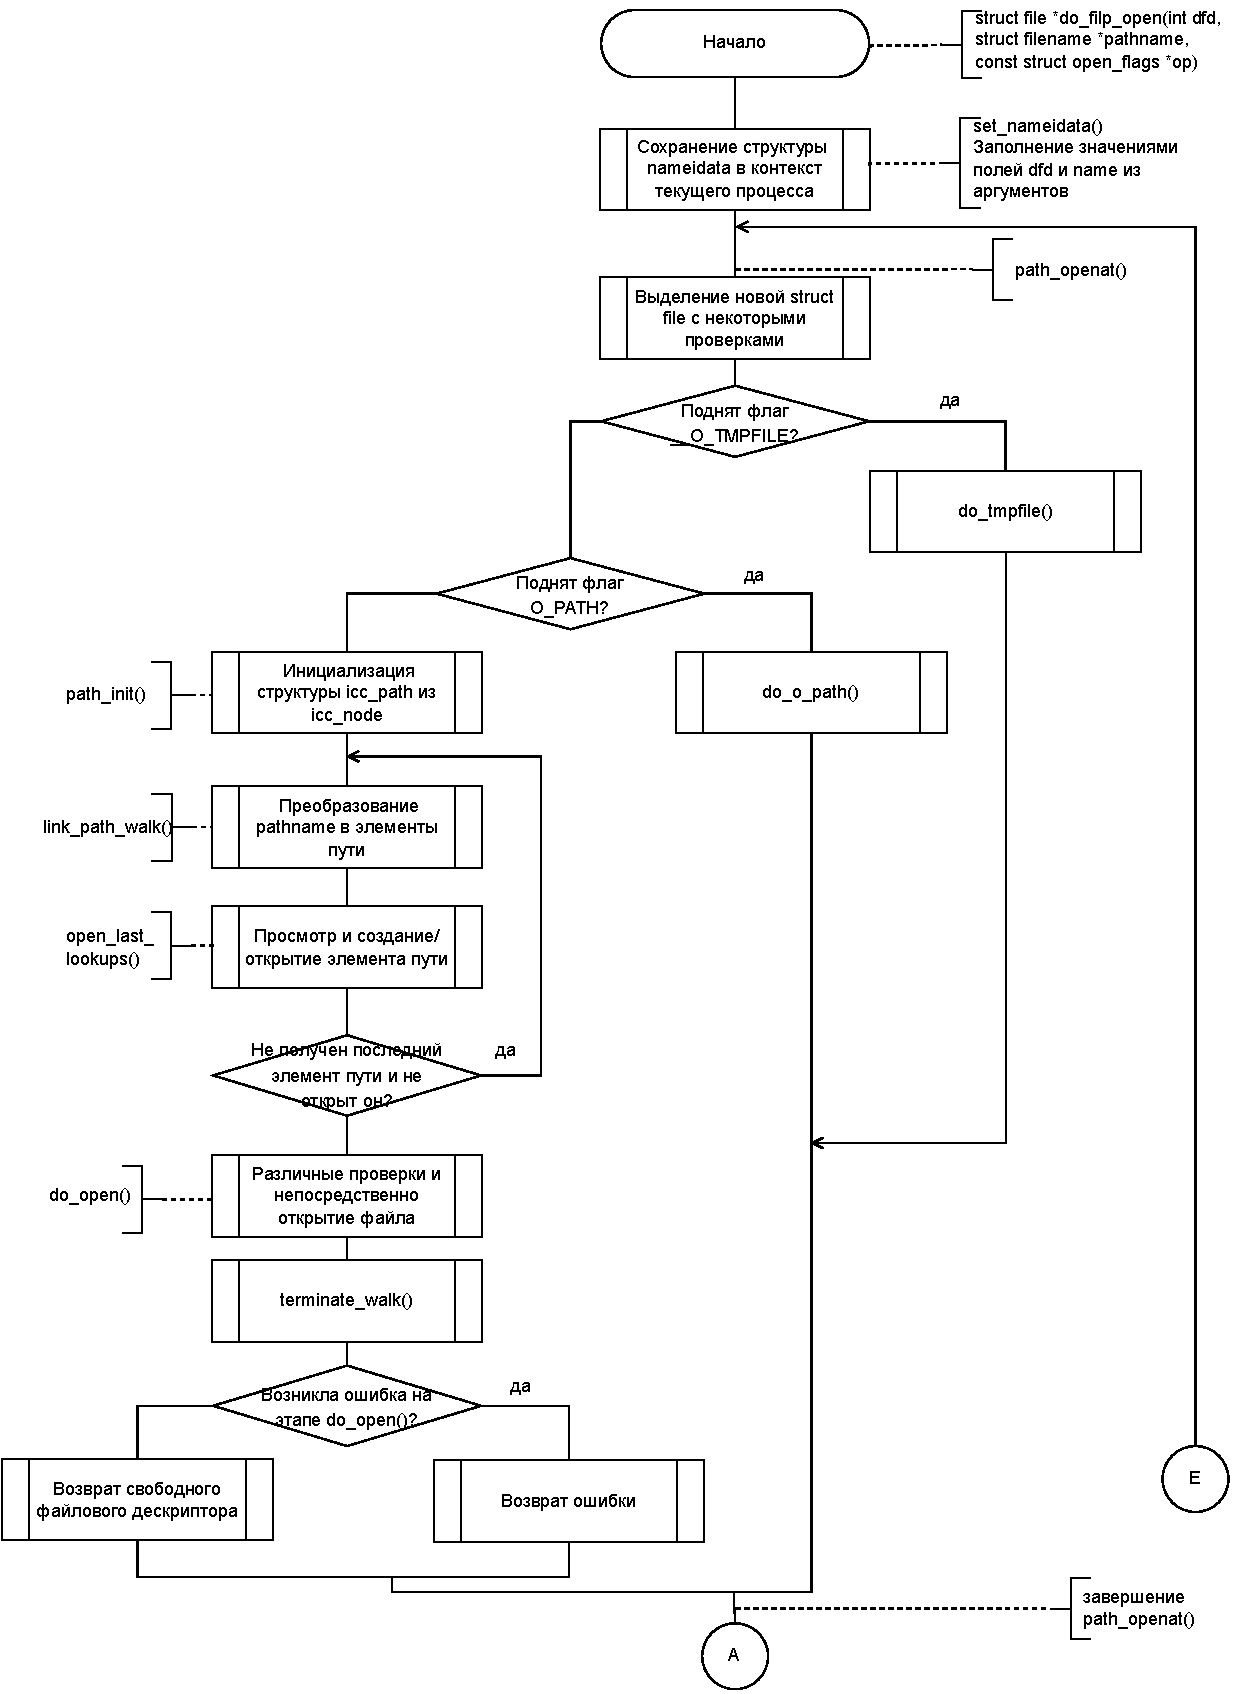
\includegraphics[scale=0.85]{images/do_filp_open_1.pdf}
		\caption{Схема алгоритма функции do\_filp\_open()}
		\label{image:do_filp_open_1}
	}
\end{figure}

\begin{figure}[H]
	\captionsetup{justification=centering}
	\centering{
		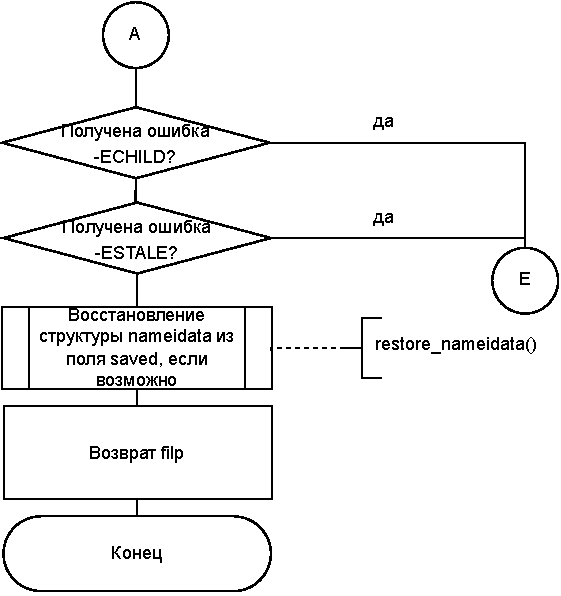
\includegraphics[scale=0.9]{images/do_filp_open_2.pdf}
		\caption{Схема алгоритма функции do\_filp\_open() (продолжение)}
		\label{image:do_filp_open_2}
	}
\end{figure}

\begin{figure}[H]
	\captionsetup{justification=centering}
	\centering{
		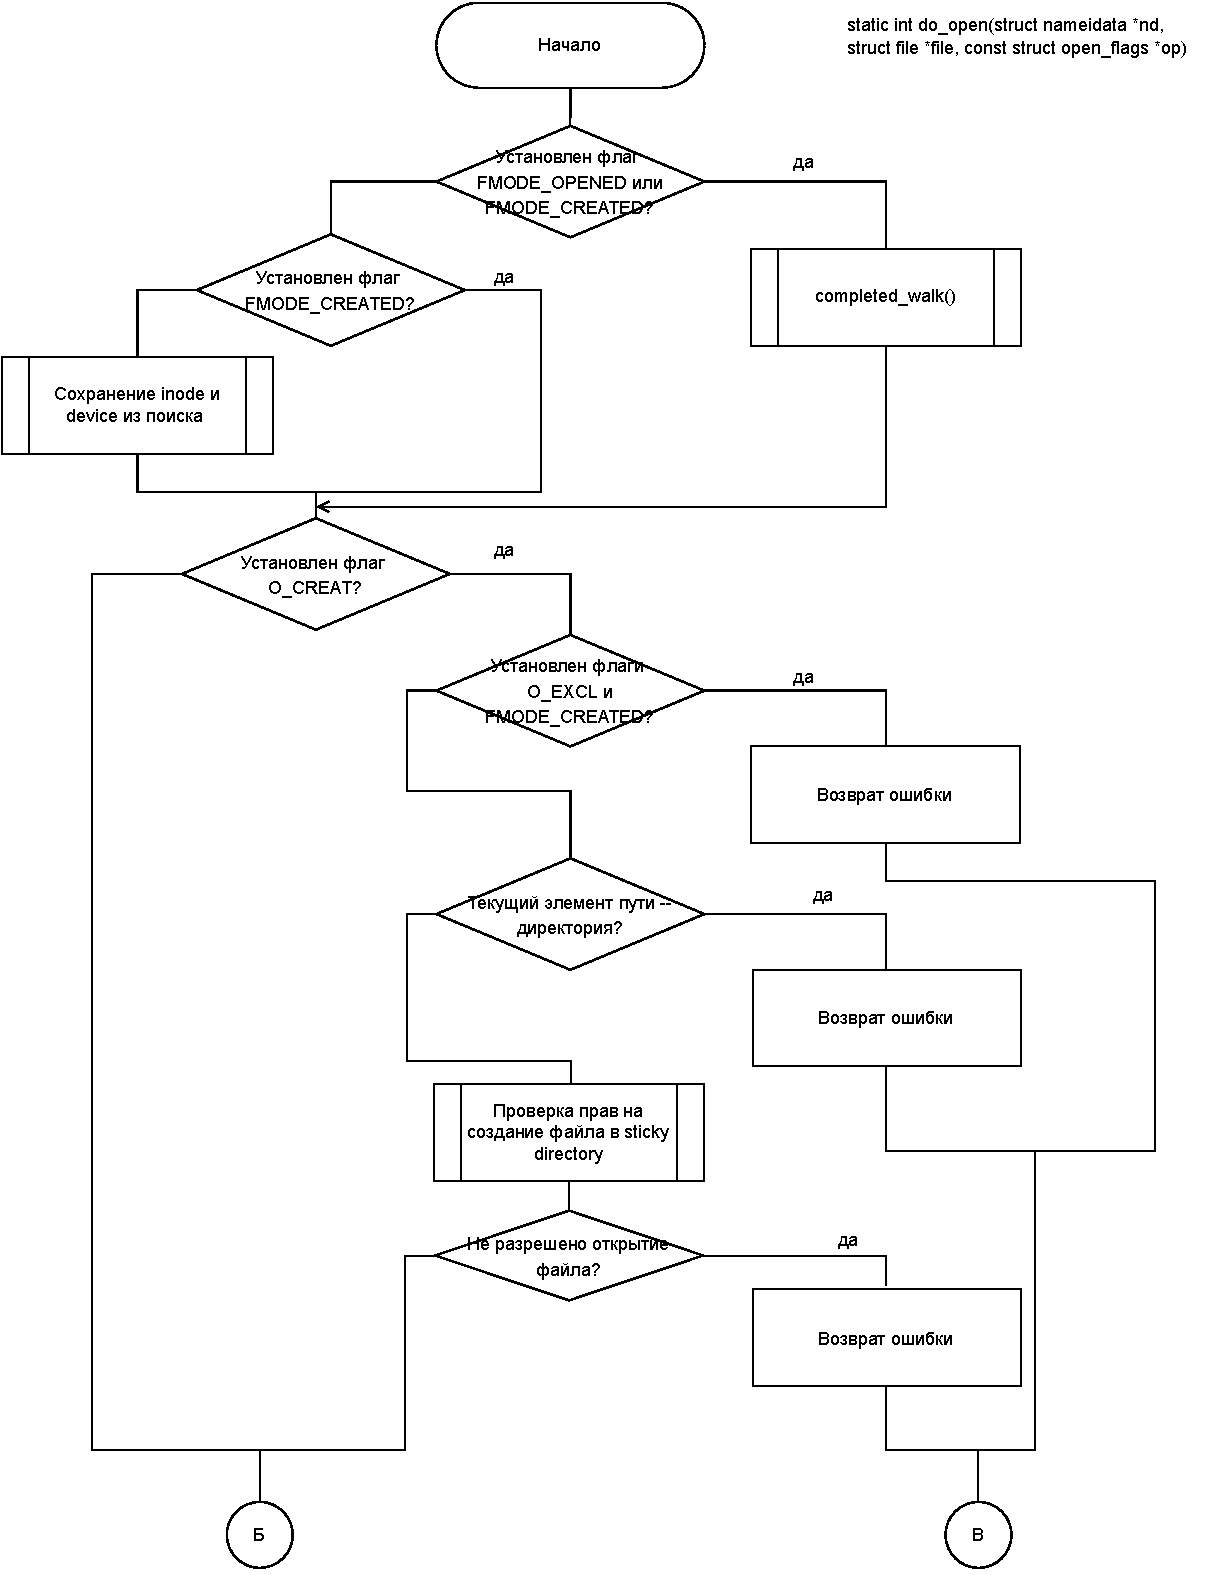
\includegraphics[scale=0.85]{images/do_open_1.pdf}
		\caption{Схема алгоритма функции do\_open()}
		\label{image:do_open_1}
	}
\end{figure}

\begin{figure}[H]
	\captionsetup{justification=centering}
	\centering{
		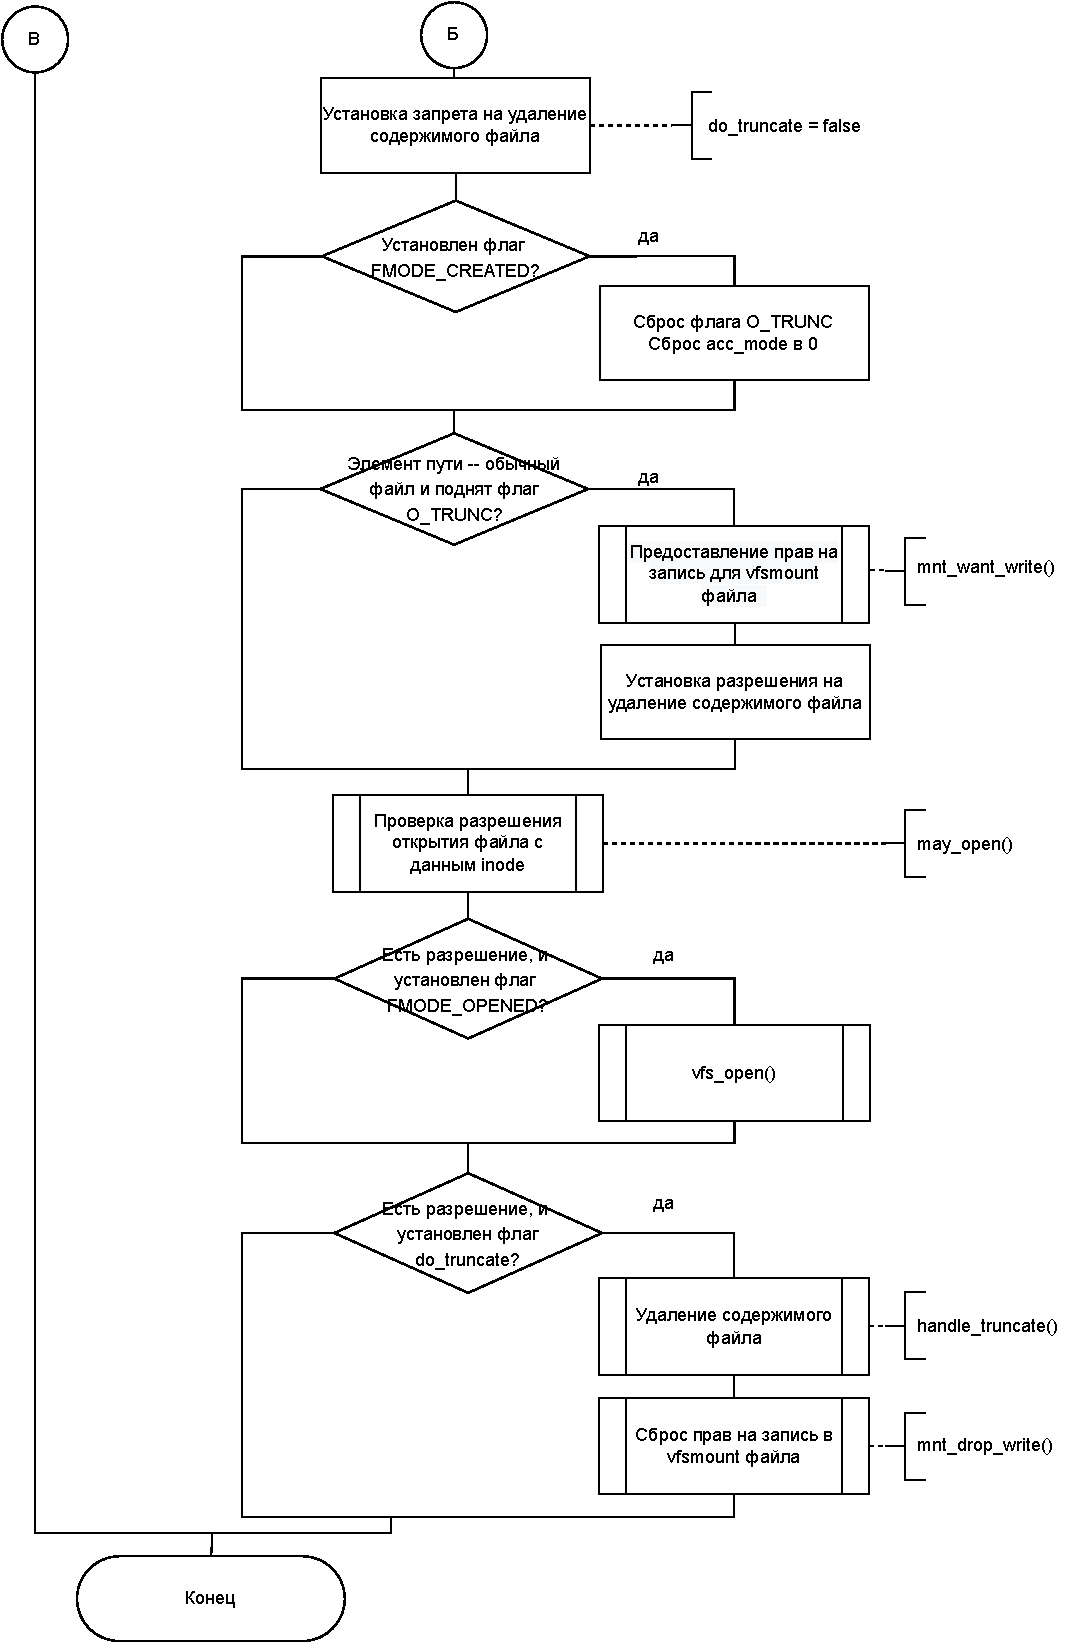
\includegraphics[scale=0.85]{images/do_open_2.pdf}
		\caption{Схема алгоритма функции do\_open() (продолжение)}
		\label{image:do_open_2}
	}
\end{figure}

\begin{figure}[H]
	\captionsetup{justification=centering}
	\centering{
		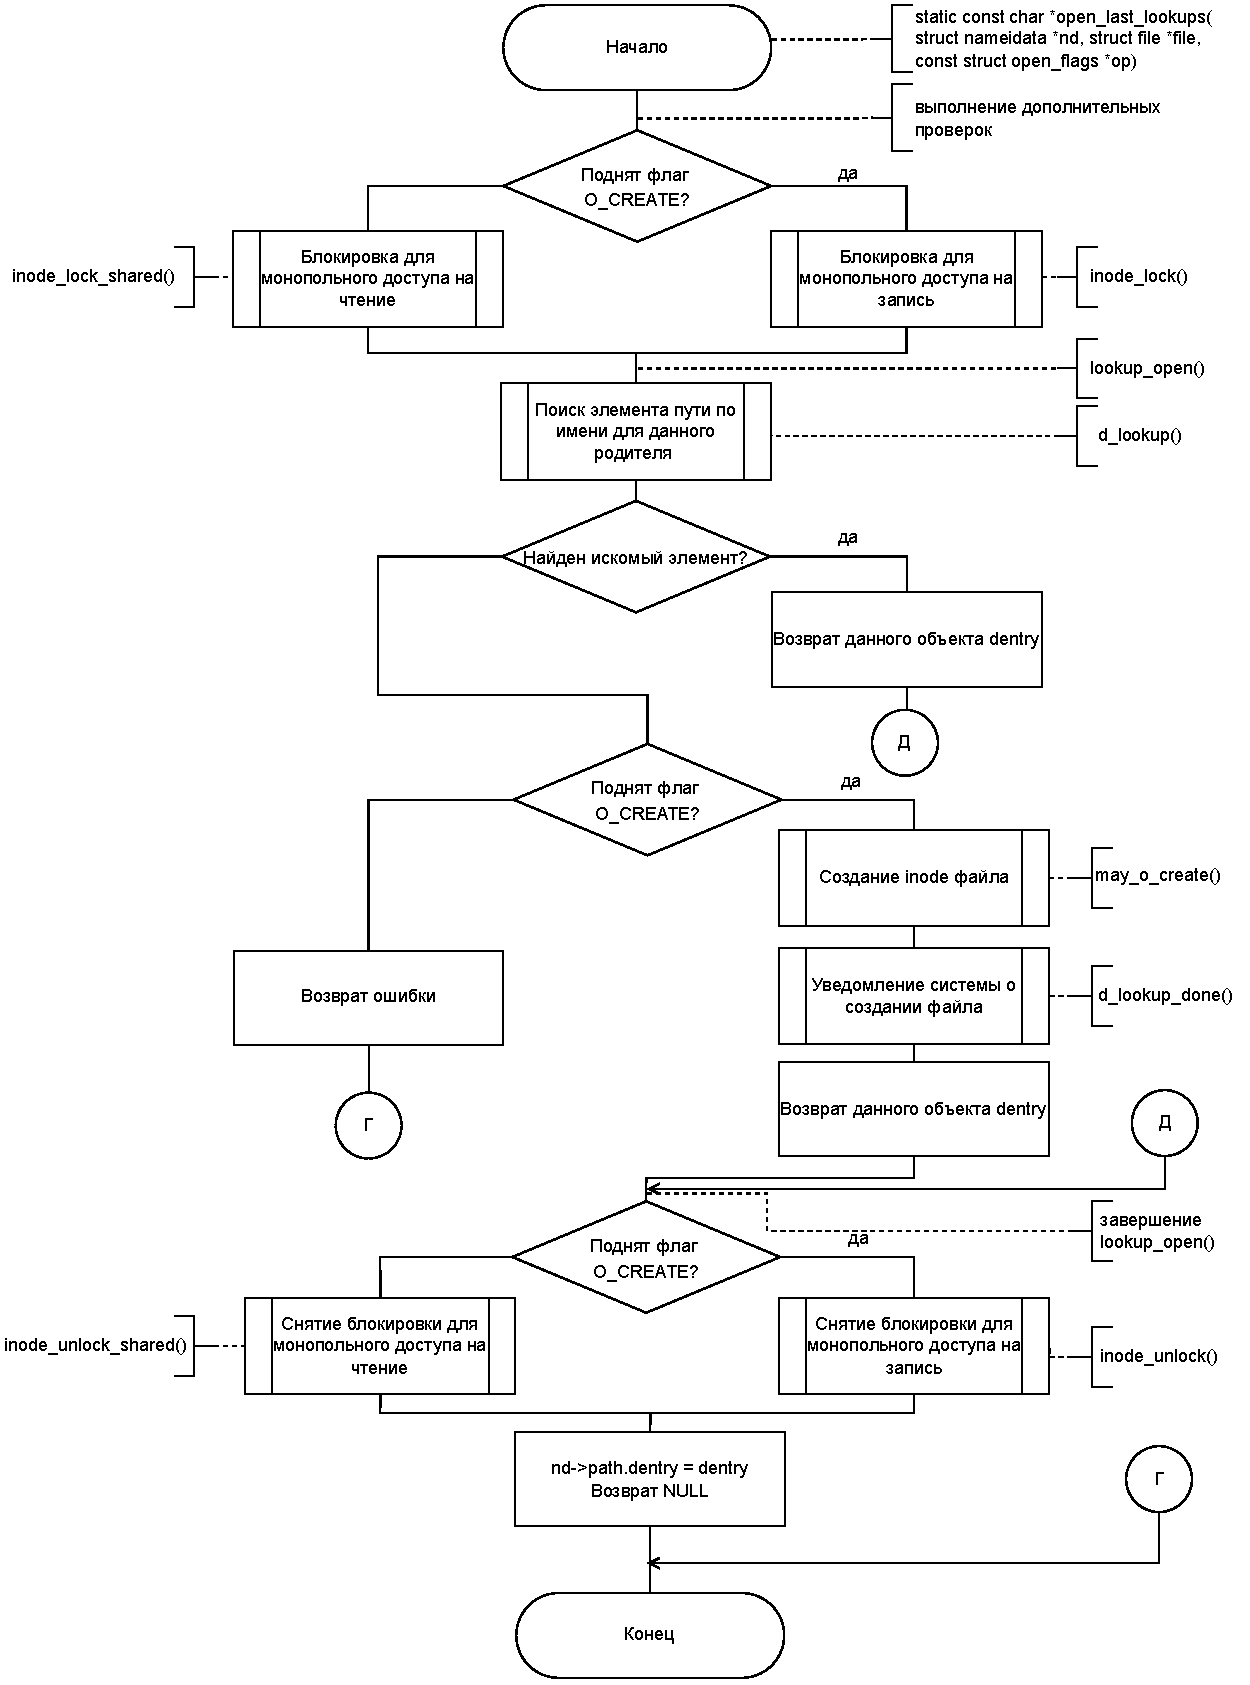
\includegraphics[scale=0.85]{images/open_last_lookups.pdf}
		\caption{Схема алгоритма функции open\_last\_lookups}
		\label{image:do_last_lookups}
	}
\end{figure}